\clearpage

\section{でんげんの切り方を覚えよう}
ruby{皆}{みな}さんのデータはmicroSDカードに\ruby{保存}{ほぞん}されています。
でんげんを急に切るとmicroSDカードに書き\ruby{込}{こ}まれる前に本体のでんげんが切れてしまい、
データが\ruby{壊}{こわ}れたりする\ruby{可能性}{かのうせい}があります。

そこで、でんげんを切る\ruby{際}{さい}は、決められた手順に\ruby{従}{したが}う必要があります。
この節ではでんげんの切り方を学びます。
ラズベリーパイを使い終わったら正しい手順ででんげんが切れるように覚えておきましょう。



\centering
\begin{figure}[H]
  \begin{minipage}{8cm}
    {\upshape
      \centering
      \includegraphics[height=4.5cm]{text01-img/textbook-img206.png}
      \caption{「ログアウト」メニュー}\label{fig:48}
    }
  \end{minipage}
  \begin{minipage}{7cm}
    図~\ref{fig:48}のようにラズベリーのアイコンをクリックすると一番下に「ログアウト」があります。
    これをクリックしてください。
  \end{minipage}
\end{figure}

\flushleft
\textcolor[rgb]{0.13333334,0.13333334,0.13333334}{図~\ref{fig:46}のような画面となったら一番上の「Shutdown」を\ruby{押}{お}してでんげんを切ります。}

\begin{figure}[H]
  \centering
  \begin{minipage}{8cm}
    {\upshape
      \includegraphics[height=4.0cm]{text01-img/textbook-img208.jpg}
      \caption{「Shutdown」画面}\label{fig:46} 
    }
  \end{minipage}  
\end{figure}

\flushleft
\textcolor[rgb]{0.13333334,0.13333334,0.13333334}{ラズベリーパイ本体の緑色のランプが消灯します。
  図~\ref{fig:47}。
  この\ruby{状態}{じょうたい}になったらでんげんアダプターをコンセントから\ruby{抜}{ぬ}きましょう。}

\begin{figure}[h]
  \centering
  \begin{minipage}{6cm}
    {\upshape
      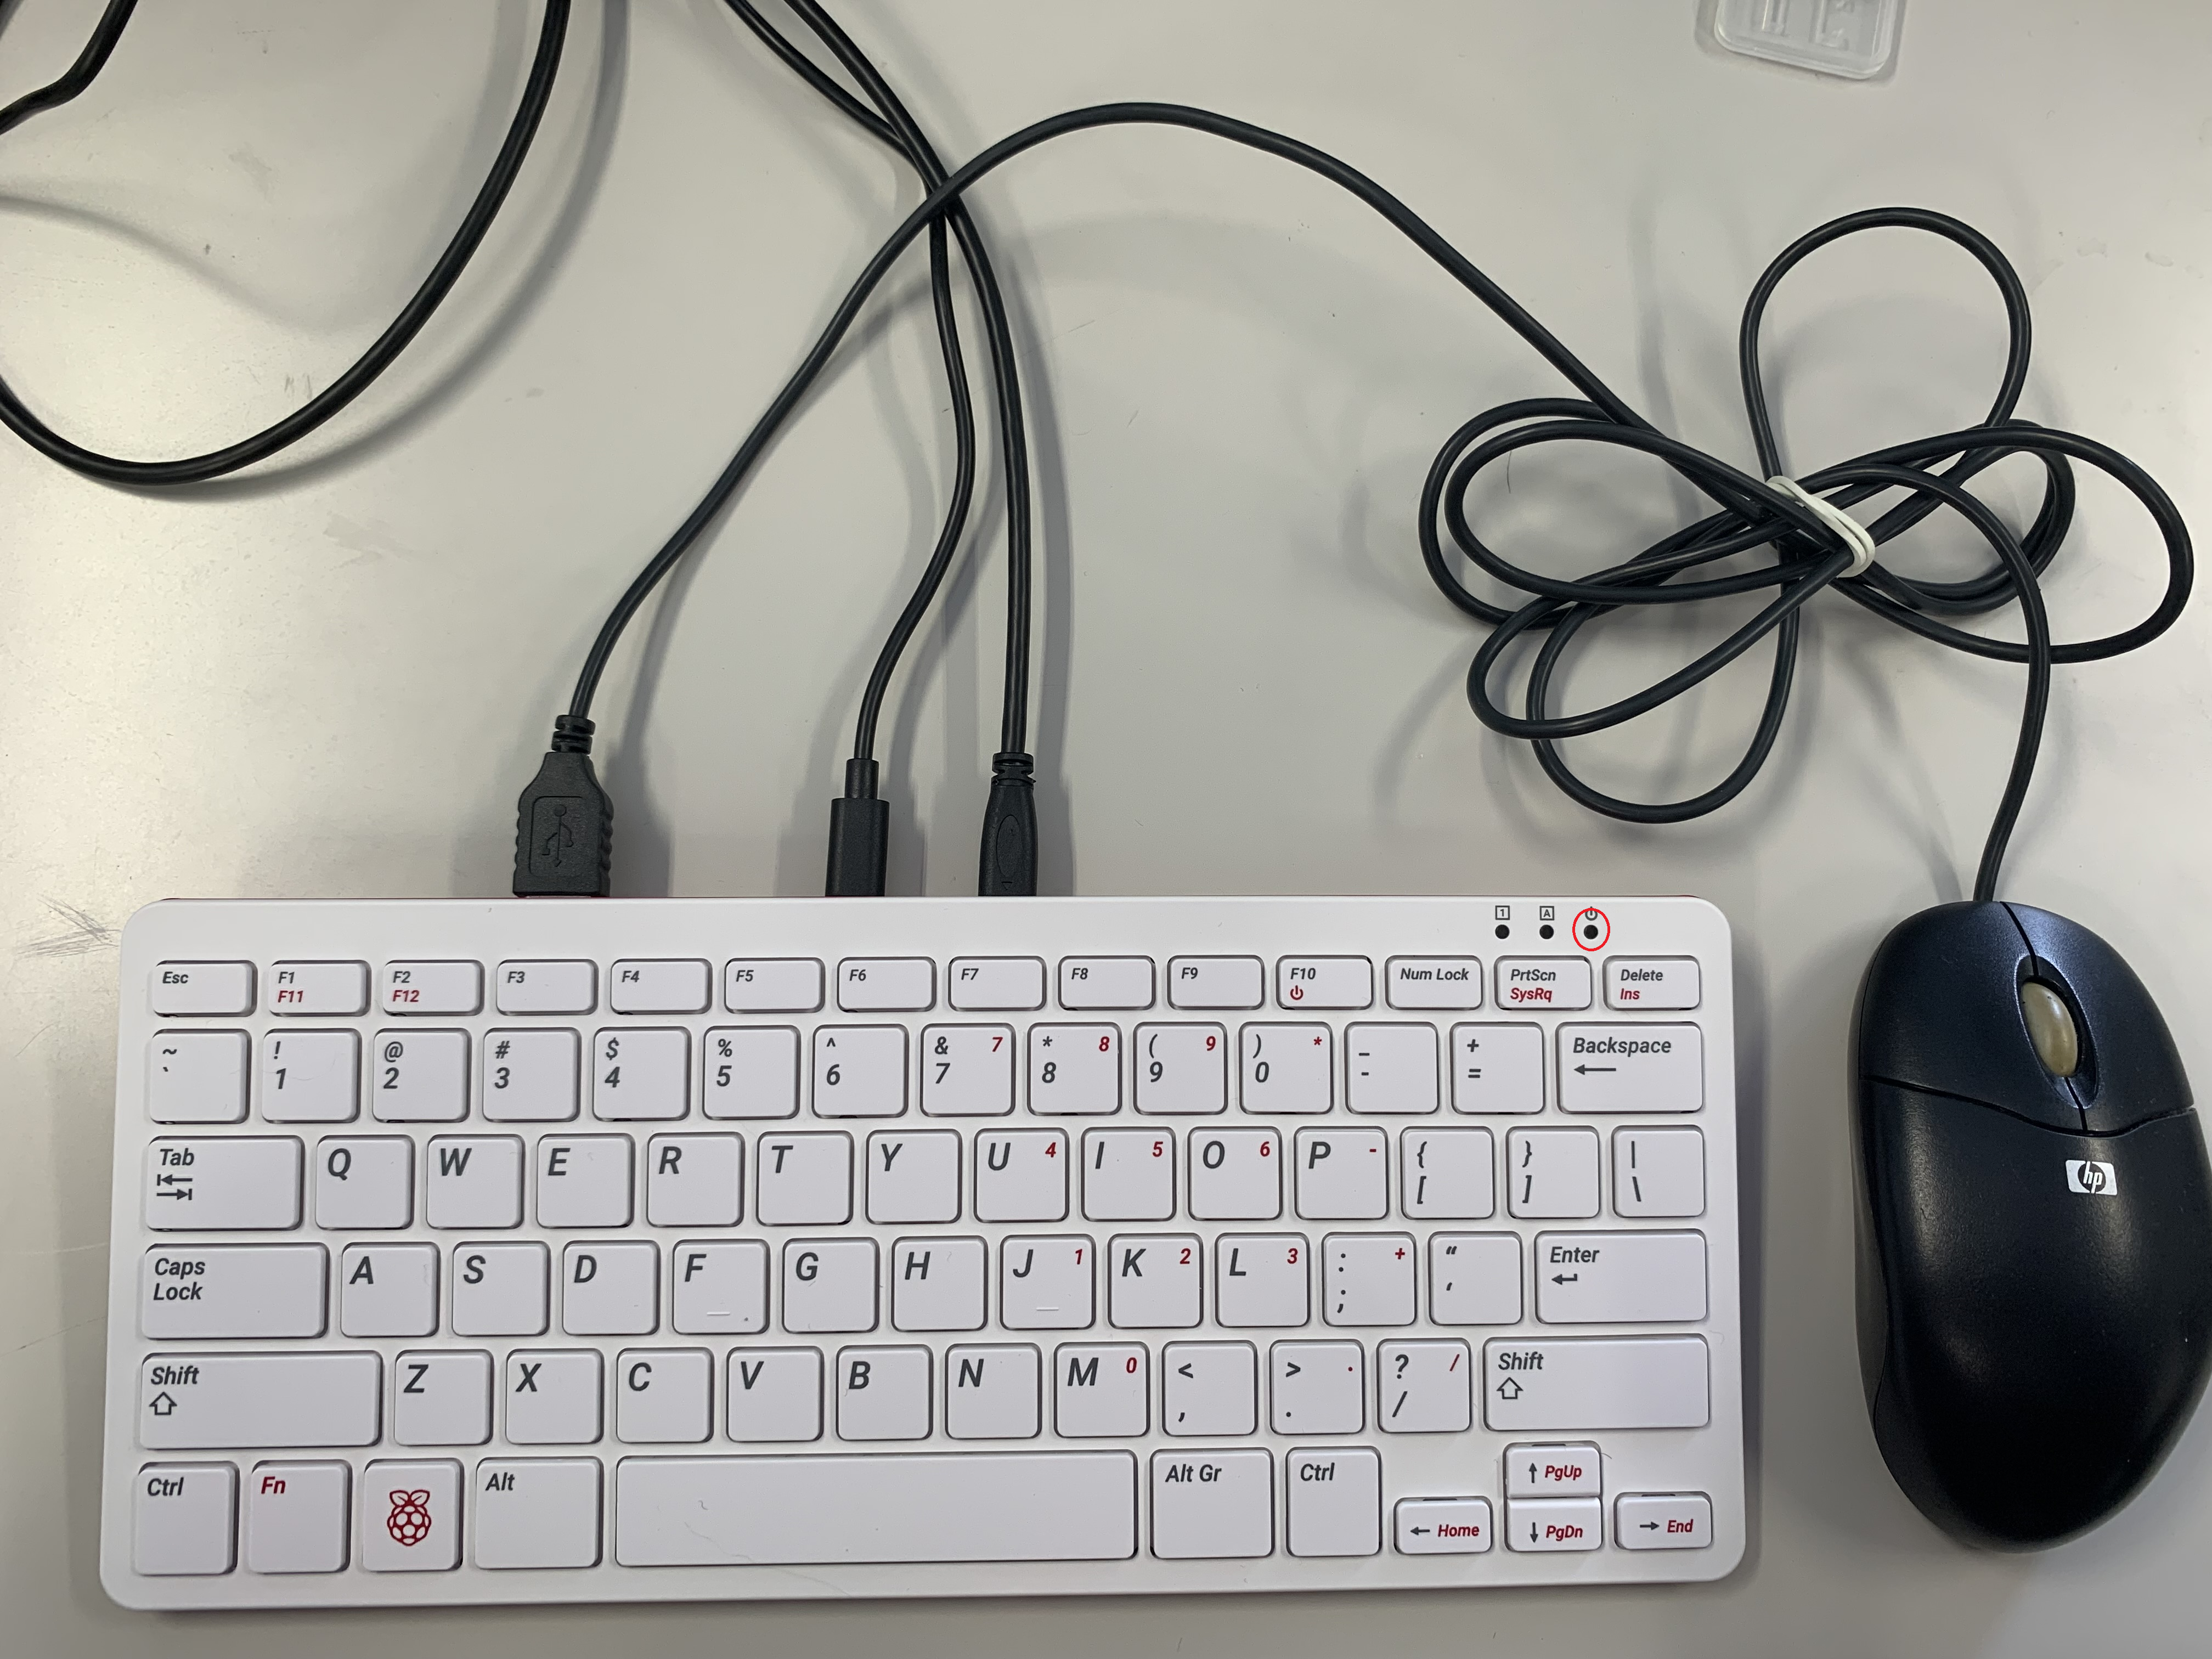
\includegraphics[height=4.5cm]{text01-img/textbook-img207-2023.png}
      \caption{Raspberry Pi ステータスランプ}\label{fig:47}
    }
  \end{minipage}
\end{figure}

\clearpage

\subsection{安全な持ち帰り方}
ラズベリーパイなどの電子機器はらんぼうに扱うと\ruby{壊}{こわ}れてしまいます。また、静電気にも弱いです。ラズベリーパイを持ち帰るときはラズベリーパイを\ruby{付属}{ふぞく}の箱へ入れて持ち帰りましょう。この箱は静電気を\ruby{防}{ふせ}いでくれます。microSDカードはなくさないようにラズベリーパイに\ruby{挿}{さ}しておきましょう。

\clearpage

